%% GENERATED by scripts/paper/build_paper.py from docs/analysis/register/findings.yaml -- do not edit by hand;
%% rewrite the prose in main.tex or change the register / scripts/paper/paper_text.json and rebuild.

\subsection{A practitioner's reading: P36, a participant with operational military experience}\label{sec:qual:practitioner}

\regtext{\textbf{Summary.} One participant had operational military experience. They played like everyone else, and differed in who they are: the oldest participant, the only one with extensive command experience, and among the most positive about AI. Their sessions and debrief are the richest material in the study, and nearly every result here has a passage of theirs that agrees with it, qualifies it or goes past it. Each point below is one passage with its own links back; the last section gathers them. This is one person's expert commentary, not evidence about the cohort; in any paper, describe them only as ``a participant with operational military experience''.} \par\noindent{\small\textit{Strength of evidence (register rating): qualitative. Your verdict: core.}}

\subsubsection{How typical are they?}\label{sec:qual:practitioner:own-play}

\noindent \passtag{numbers only} \usernote{Your note: We will say that our expert was a good performer with a slightly higher workrate than others, prempting cards more, but was otherwise fairly typical (insert a couple numbers into here)}

\noindent \regtext{\textbf{Typical in how they played.} On every habit the findings measure (card use, how card use grows with mission size, Suggest use and how it grows with plan size, keeping Suggest plans unedited, the drones on a hand build, oldest-first) they sit in the middle half of the cohort. They were a little quicker on the strategic step (9.6 s per decision against a median of 11.4) and decided before the cards loaded a little more often (32\% against 10\%), at the 20th and 80th percentiles, and they scored a little above most (0.7 SD within game, 80th percentile). \textbf{Different in who they are.} They are the oldest participant (44; median 27), the only one with extensive command experience (24 of 33 report none), one of four with moderate drone experience, at the top of the AI-attitude scale (10 of 10, with one other), and among the least insistent that a human keep authority (3.0 against a median of 4.3). Their trust in the Strategic Assistant was higher than most (5.9; median 4.5). So the commentary that follows comes from someone whose play was ordinary: what they add is the reading, not a different way of playing.} (Figure~\ref{fig:qual:practitioner:own-play})

\begin{figure}[H]
\centering
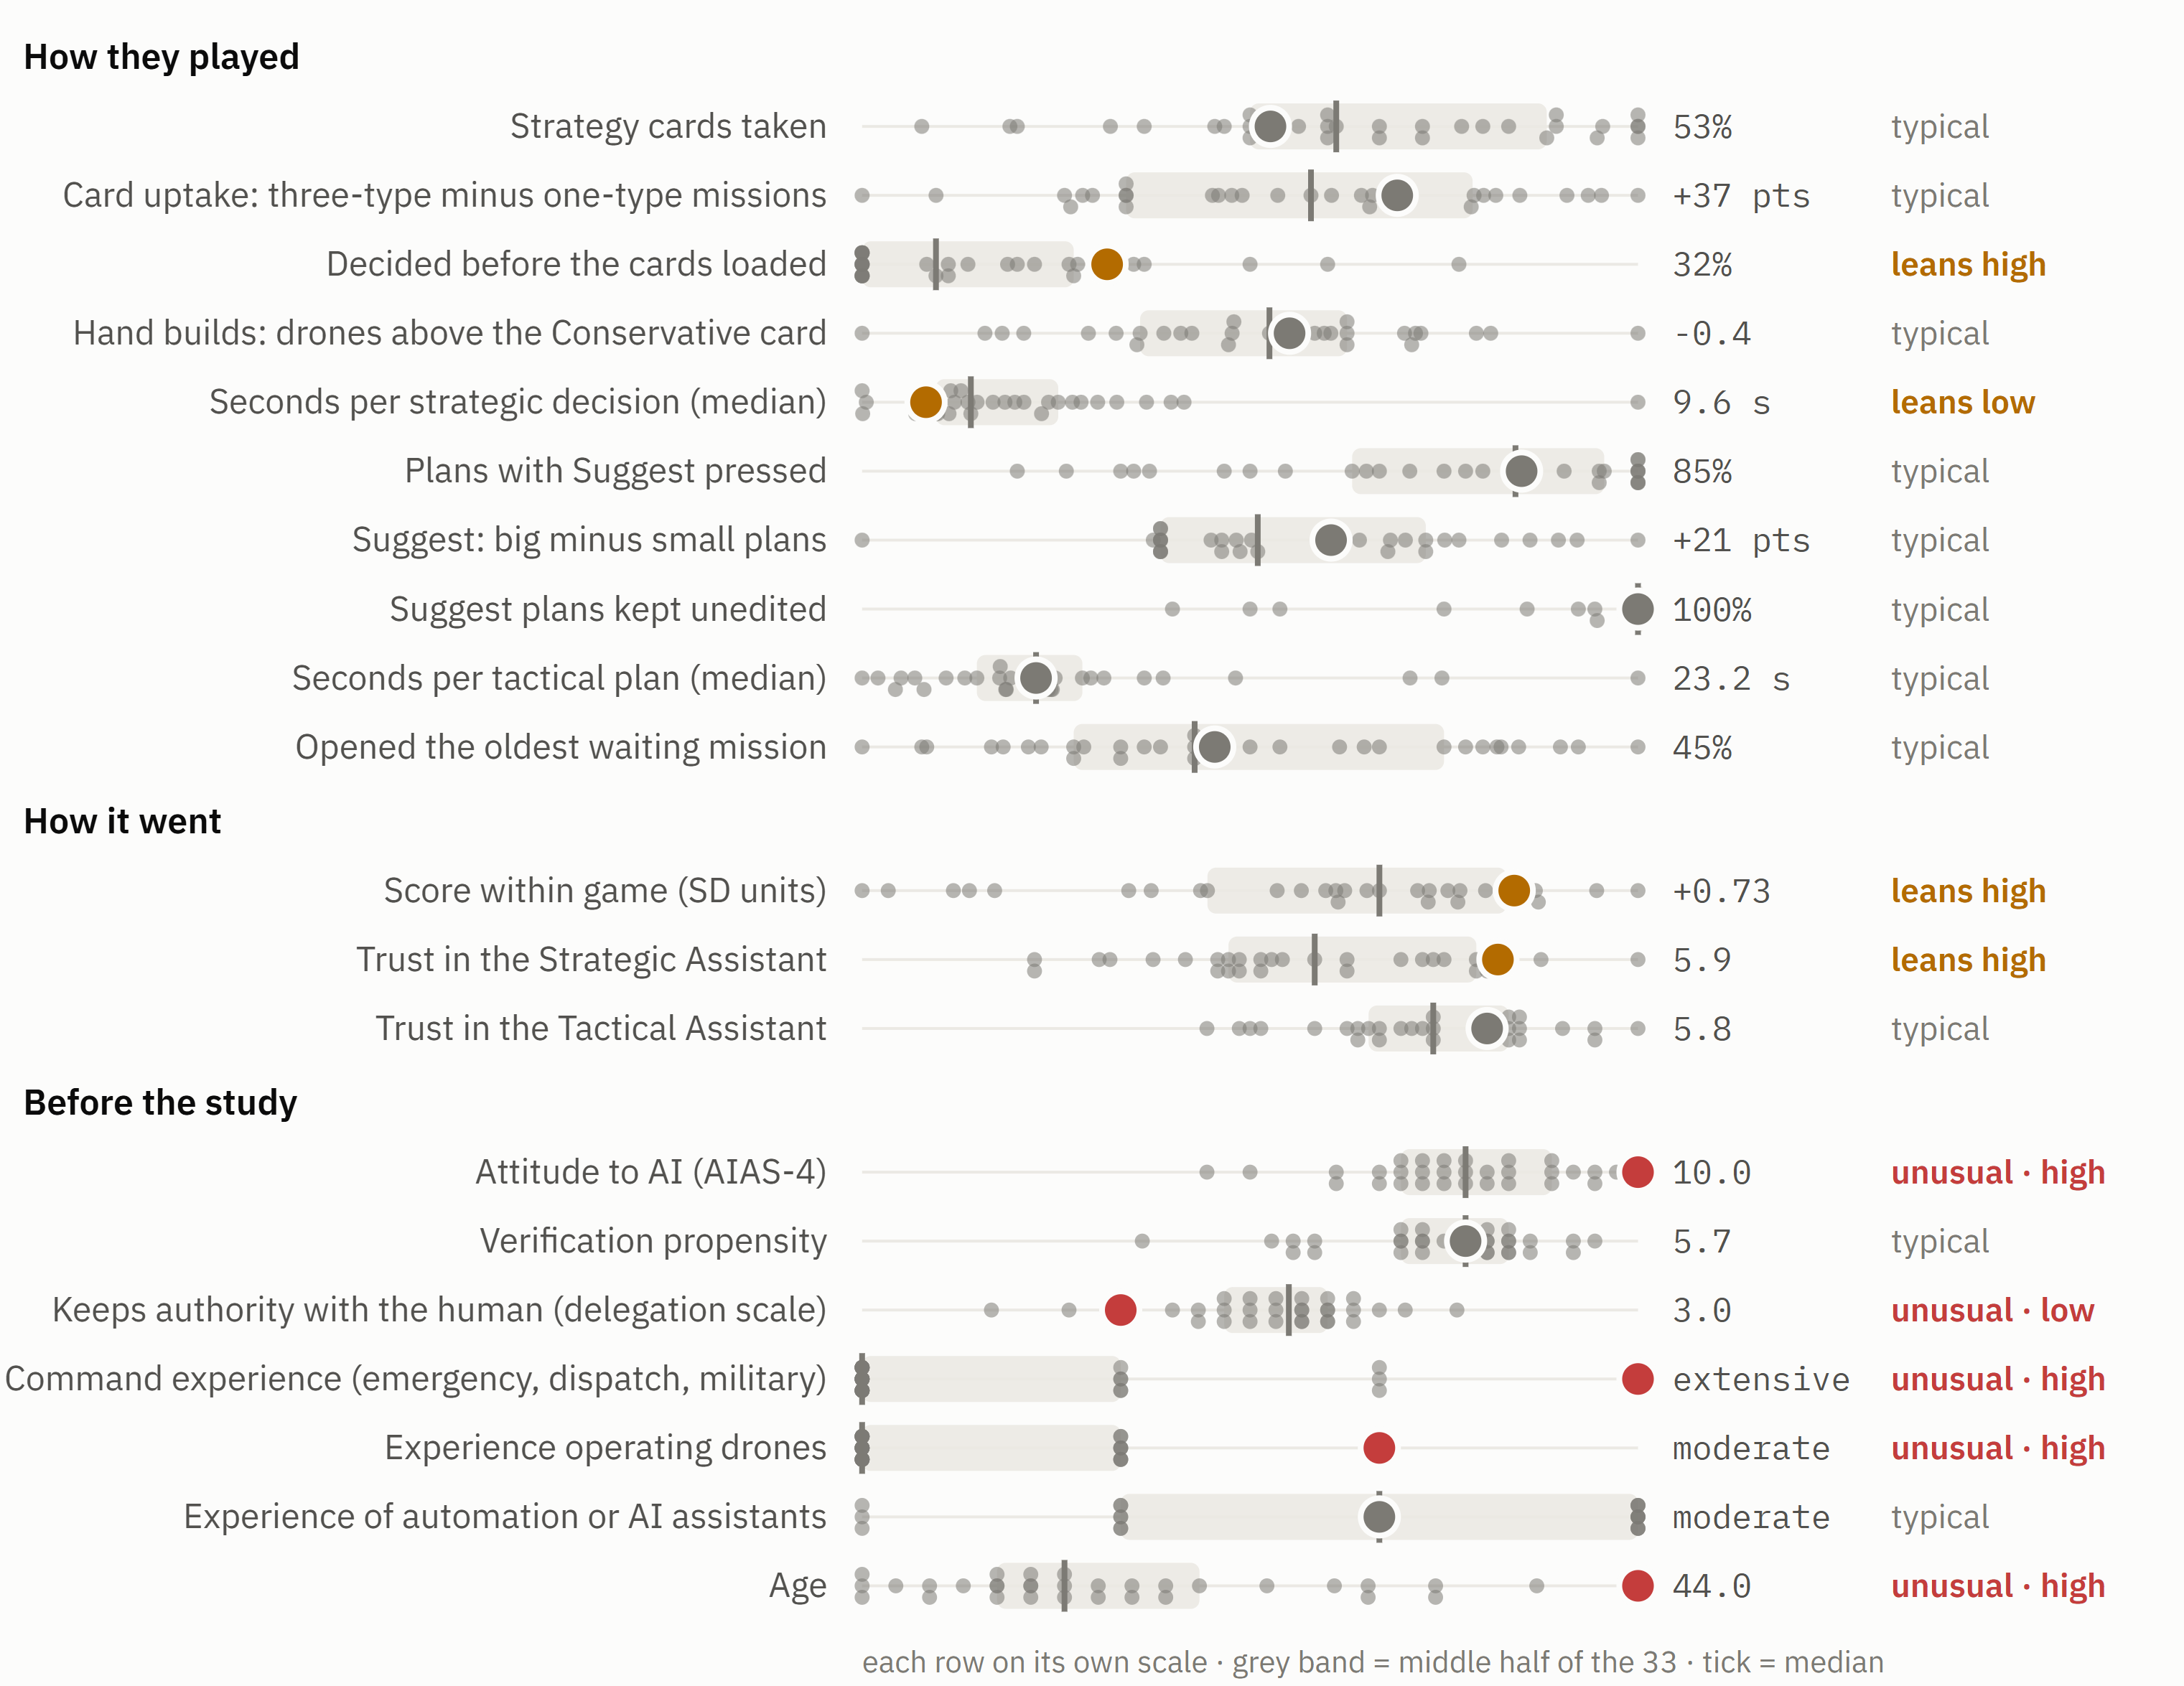
\includegraphics[width=\linewidth,height=0.55\textheight,keepaspectratio]{figs/results/q-practitioner__own-play__main.png}
\caption{\textbf{How typical are they?}}
\label{fig:qual:practitioner:own-play}
\end{figure}

\paragraph*{Method.} {\small One value per person for each measure (33 people, P09 excluded): play habits from the same per-person table as the size and speed findings, oldest-first from the queue choice decisions, trust as the mean of the session ratings, and the pre-study questionnaire (experience items scored none 0 to extensive 3). P36's percentile rank among the 33 (ties share the middle). Typical = middle half; leans = 10th--25th or 75th--90th; unusual = beyond. With one person nothing is tested; this only places them. scripts/register/pass2/typical.py; results in pass2/typical.json.}

\clearpage

\subsubsection{How they played: for the whole board, not the mission}\label{sec:qual:practitioner:pt-whole-board}

\noindent \passtag{for the paper} \usernote{Your note: We'll briefly quote the second part I think}

\noindent \regtext{Five minutes in, P36 states the aim as throughput across every task while watching the reserve (``running a little bit low on blue''), and later gives the reason: ``success is generated across all of the tasks rather than just an individual task''. The two passages make one point, so they share it. This is the cross-mission view operators said the cards lack, and it fits the cohort's hand builds, which mostly sit at or below the cards.}

\paragraph*{Quotes selected for this section.}

\begin{quotelist}

\item ``so generally speaking all I'm trying to do here is get as many across as quickly as I can to complete all of the tasks managing my resources that I've got left here so I'm running a little bit low on blue over there and then just double checking on here so I've got the redundancy in there''\,---\,P36 (think-aloud s1 0:05:32)\par\usernote{Your comment: Minor}

\item ``so when I think it's going to be quicker because it's not necessarily about just that task it's about all of the tasks and success is generated across all of the tasks rather than just an individual task.''\,---\,P36 (think-aloud s1 0:05:58)\par\usernote{Your comment: Interesting}

\end{quotelist}

\paragraph*{Links back to the results.}

\begin{itemize}[leftmargin=1.2em,itemsep=1pt]\small
\item \textit{Agrees with} Section~\ref{sec:res:size-decides:parallel}, \emph{Where the tactical time goes: hand-built and Suggest plans are close, with a small edge to Suggest in carrying the plan out}: Their aim is throughput across the board (``get as many across as quickly as I can to complete all of the tasks''), the same reason the cohort gives for starting Suggest and moving on.
\end{itemize}

\paragraph*{Links back to the results.}

\begin{itemize}[leftmargin=1.2em,itemsep=1pt]\small
\item \textit{Agrees with} Section~\ref{sec:qual:hierarchy:cross-mission}, \emph{The cross-mission view the cards lack}: Operators overrode the cards to act on what one mission's card cannot see. P36 says why in one line: ``success is generated across all of the tasks rather than just an individual task''.
\item \textit{Agrees with} Section~\ref{sec:res:manual-cards:dots}, \emph{Each manual decision against the Conservative card}: Playing for every task shows in the cohort's hand builds: on 44\% of decisions they sit below both cards, mostly by leaving off the card's spare, which keeps drones for the next mission.
\end{itemize}

\clearpage

\subsubsection{How they played: the card can be slower than doing it yourself}\label{sec:qual:practitioner:pt-quicker-by-hand}

\noindent \passtag{extra: may make it in}

\noindent \regtext{Three minutes into the first session, after taking a card on a small mission, P36 decides it would have been quicker by hand. It is the speed result in miniature: the card saves time only on big, three-type jobs.}

\paragraph*{Quotes selected for this section.}

\begin{quotelist}

\item ``Do you know what? Probably quicker just to hit three on there. But we'll go three on that one there. [\ldots{}] I probably should have done that one manually. It would have been quicker.''\,---\,P36 (think-aloud s1 0:03:21)

\end{quotelist}

\paragraph*{Links back to the results.}

\begin{itemize}[leftmargin=1.2em,itemsep=1pt]\small
\item \textit{Agrees with} Section~\ref{sec:res:size-decides:speed}, \emph{Why the rule makes sense: the card pays only on big strategic jobs; Suggest is not slower}: The card saves time only on big three-type jobs. Three minutes into their first session P36 finds it out: ``Probably quicker just to hit three'', then ``I probably should have done that one manually. It would have been quicker.''
\end{itemize}

\clearpage

\subsubsection{How they played: simple by hand, complex to the assistant, and why}\label{sec:qual:practitioner:pt-branching-paths}

\noindent \passtag{for the paper} \usernote{Your note: This one is a new idea that we can talk about in more depth in the paper: More complicated tasks can have a more branching failure space. This is not something we cover in this work, but could be an important factor in future works.}

\noindent \regtext{The fullest statement of the size rule in the study, with both halves of the reason. On a simple mission they already know the answer by eye, and they build in redundancy (every drone to every task) so that after a failure ``you don't really need to change the story''. On a complex one the options branch, so they let the assistant start and step in when needed. They also name the limit of the quick check that goes with handing over: whether it is right ``is another question entirely''. Their own log follows the rule.}

\paragraph*{Quotes selected for this section.}

\begin{quotelist}

\item ``sometimes it's going to be a little bit uh quicker to do these myself only because i know the answer based on what i'm seeing visually in front of me so i don't need to do that much [...] simple task you probably want to do yourself if you're going to get the solution quicker and the more complex tasks you're going to want somebody to give you that solution in front of you so you can give it a quick once over and go that looks about right um whether or not it is right of course it's another question entirely [...] the solutions it is coming up with uh i would have to go and do a much more thorough scan of the solution to say have you put redundancy into that plan or do i care like i've put redundancy into that plan so i don't have to come back to it i've put every turn on that last blue one every single drone is going to every single task so that if one of my drones fails my assumption is that my other drones are picking up the task whereas the more complex ones just literally looking have they allocated enough to that task started going because if it fails um think about like hypertextual branching paths so as soon as i get one failure that's going to change the entire story how much of that story do we need to change on the blue ones you don't really need to change the story you're just going to flick through whereas the other ones it's like okay no i've got more options so my option scope is broader and so it's going to need more human intervention to go into it so there's no point in me trying to think about all of that ahead of time i may as well let them start on that task and then intervene when i need to''\,---\,P36 (think-aloud s1 0:09:12, includes the researcher's words)

\end{quotelist}

\paragraph*{Links back to the results.}

\begin{itemize}[leftmargin=1.2em,itemsep=1pt]\small
\item \textit{Agrees with} Section~\ref{sec:res:size-decides:both}, \emph{Both tiers on one axis: the bigger the mission, the more it is handed over}: Small jobs by hand, big jobs to the assistant (cohort: card 56\% to 75\%, Suggest 54\% to 91\%). P36 gives both halves of the reason: on a simple job ``i know the answer based on what i'm seeing visually'', and a failure needs no re-plan (``you don't really need to change the story''); on a complex one ``my option scope is broader'', so ``let them start on that task and then intervene when i need to''. Their own log follows it (card 33\% to 70\%, Suggest 79\% to 100\%).
\item \textit{Agrees with} Section~\ref{sec:res:tier-trust:checking}, \emph{Why the tactical plan is kept: checking it is brief and does not grow with the plan}: ``Give it a quick once over and go that looks about right ... whether or not it is right of course it's another question entirely'': the brief check the timing data show, with its limit named.
\item \textit{Agrees with} Section~\ref{sec:qual:hierarchy:one-plan}, \emph{One plan across both decisions}: P21 chained drones through each other's tasks for ``redundancy for free''. P36 does the same on simple missions (``every single drone is going to every single task so that if one of my drones fails ... my other drones are picking up the task''), which is why those plans need no checking afterwards.
\end{itemize}

\clearpage

\subsubsection{How they played: the rule bends when the reserve is full}\label{sec:qual:practitioner:pt-resource-rich}

\noindent \passtag{extra: may make it in} \usernote{Your note: minor, may make it in}

\noindent \regtext{A simple mission, so by their own rule one to do by hand; but the reserve is full and nothing is coming in, so they press Suggest anyway. The size rule is a default, not a law, and slack loosens it. It also cuts against the idea that people hand over because they are busy: here they hand over because they are not.}

\paragraph*{Quotes selected for this section.}

\begin{quotelist}

\item ``so again this one here that's relatively simple and I'm resource rich at the moment so we'll go nuts I'll start suggesting some stuff through because there's nothing else that's coming in''\,---\,P36 (think-aloud s2 0:20:33)

\end{quotelist}

\paragraph*{Links back to the results.}

\begin{itemize}[leftmargin=1.2em,itemsep=1pt]\small
\item \textit{Qualifies} Section~\ref{sec:res:size-decides:both}, \emph{Both tiers on one axis: the bigger the mission, the more it is handed over}: The size rule bends with slack: this mission is ``relatively simple'', but ``I'm resource rich at the moment so we'll go nuts I'll start suggesting''.
\item \textit{Agrees with} Section~\ref{sec:res:workload:raw-vs-adjusted}, \emph{Queue depth against reliance --- raw, and adjusted}: A busier moment does not push people onto the assistants. P36 presses Suggest at a quiet moment, ``because there's nothing else that's coming in''.
\end{itemize}

\clearpage

\subsubsection{How they played: oldest first, and never without a reserve}\label{sec:qual:practitioner:pt-reserve}

\noindent \passtag{for the paper} \usernote{Your note: Short note - they identified an classified a rule ``never without a reserve''. Links to the consistency factor in training.}

\noindent \regtext{Two of the cohort's habits in one sentence: open the mission that has waited longest unless something changes the priority, and build by hand with a spare (``minimum two, we're going to go three''). Their builds still land where the cohort's do relative to the cards.}

\paragraph*{Quotes selected for this section.}

\begin{quotelist}

\item ``this one's been there for the longest i've got nothing in there that's going to change my prioritization so i'm going to go into here and probably send manually i'm going to give you minimum two we're going to go three just never deploy without a reserve''\,---\,P36 (think-aloud s1 0:07:50)

\end{quotelist}

\paragraph*{Links back to the results.}

\begin{itemize}[leftmargin=1.2em,itemsep=1pt]\small
\item \textit{Agrees with} Section~\ref{sec:res:triage:order}, \emph{Order: still oldest-first well above chance}: Operators open the oldest waiting mission well above chance. P36: ``this one's been there for the longest i've got nothing in there that's going to change my prioritization''.
\item \textit{Qualifies} Section~\ref{sec:res:manual-cards:dots}, \emph{Each manual decision against the Conservative card}: Most of the cohort's hand builds sit at or below the cards (44\% below both). P36 adds a spare on purpose (``minimum two we're going to go three just never deploy without a reserve''), yet their builds land where the cohort's do: on average 0.4 of a drone under the Conservative card, against a median of 0.6 under.
\end{itemize}

\clearpage

\subsubsection{How they played: critical tasks over score}\label{sec:qual:practitioner:pt-critical-first}

\noindent \passtag{for the paper} \usernote{Your note: good}

\noindent \regtext{Out of Fast drones, they accept a lower score to get the critical tasks done, ``if this is a real life scenario''. The cohort leans the same way, opening the more critical waiting mission more often; P36 says the trade aloud and frames it as what a real operation would demand.}

\paragraph*{Quotes selected for this section.}

\begin{quotelist}

\item ``i've run out of blue so that's gonna hurt my score but at the same time i've got the critical tasks done so i'd rather do the critical tasks if this is a real life scenario i'd rather be focused on the critical tasks than getting those done to a higher value rather than moderate tasks of getting them done to a low''\,---\,P36 (think-aloud s1 0:07:50)

\end{quotelist}

\paragraph*{Links back to the results.}

\begin{itemize}[leftmargin=1.2em,itemsep=1pt]\small
\item \textit{Agrees with} Section~\ref{sec:qual:new-jobs:queue-order}, \emph{An assistant for what to open next}: Operators lean towards the more critical waiting mission ($\times$1.45 per category, on top of oldest-first). P36 goes further and spends score on it: ``i've run out of blue so that's gonna hurt my score but ... i'd rather do the critical tasks if this is a real life scenario''.
\end{itemize}

\clearpage

\subsubsection{How they played: trusting the strategy card more, then seeing why that is a risk}\label{sec:qual:practitioner:pt-strategic-trust}

\noindent \passtag{extra: may make it in}

\noindent \regtext{One of the few who trusted the Strategic Assistant more than the Tactical, and their ratings say the same. The reason is that checking a card is easy (is there a reserve?), and a strategic mistake seemed less costly; then, mid-sentence, they reverse it: a bad allocation at the start leaves the tactical step ``screwed''. Easy to check is not the same as low stakes.}

\paragraph*{Quotes selected for this section.}

\begin{quotelist}

\item ``the strategic one i was less concerned about the solutions it presented so i hesitated less on the strategic than the tactical but only because all i was looking at there was have i got a reserve allocated whereas a tactical one it's 'have you covered all the tasks' and there is a reserve [\ldots{}] I wouldn't trust any of them without checking but I trust the strategic slightly more because the consequences are slightly - less they're probably not actually are they if you fuck up the allocation at the start of it then you're screwed going into the tactical''\,---\,P36 (talk during the questionnaire survey1 0:13:46)

\end{quotelist}

\paragraph*{Links back to the results.}

\begin{itemize}[leftmargin=1.2em,itemsep=1pt]\small
\item \textit{Qualifies} Section~\ref{sec:res:tier-trust:gap}, \emph{Trusted more: the basic result}: The cohort trusts the Tactical Assistant more; P36 is one of the exceptions, and their ratings match what they say (``I trust the strategic slightly more'': 5.9 against 5.8 on the 1--7 scale, where the cohort's median strategic rating is 4.5). They hesitated less over the cards only because ``all i was looking at there was have i got a reserve allocated''.
\item \textit{Agrees with} Section~\ref{sec:qual:hierarchy:cascade}, \emph{The strategic step carries the risk}: P19 put the only remedy for failures with the strategic tier. P36 reaches the same point in mid-sentence, and it reverses their reason for trusting the cards: ``they're probably not actually are they if you fuck up the allocation at the start of it then you're screwed going into the tactical''.
\end{itemize}

\clearpage

\subsubsection{The task: physics sets the pace, and the load moves to waiting}\label{sec:qual:practitioner:pt-physics-pace}

\noindent \passtag{for the paper}

\noindent \regtext{The game's pace is not realistic: real drones are bounded by distance and speed, so decisions get faster but the operation does not. The load does not go away; it becomes waiting and contingency planning (``what am I going to do if this thing fails''), ``loaded in a slightly different way''.}

\paragraph*{Quotes selected for this section.}

\begin{quotelist}

\item {\upshape\footnotesize Researcher: so I would ask in your professional opinion obviously this is clearly we're trying to get at something that we think is of interest in this kind of setting and stuff in reality I'd imagine the strategic and tactical thing would probably be done by two people but how relevant would you say this kind of set up is}\par ``so in terms of delivery absolutely in terms of the pace probably not so much [...]if you think so the biggest thing for us that is always hard to convey to decision makers is: physics remains the bounding factor I've got to get from this point here to that point there and if the adversary can see me from 20k away then I'm doing that activity from 20k and if you're going at 3k an hour then that's going to take you a long time to get from here to over there so there's a level of that acceleration in terms of decision however on the flip side of it when the shit hits the fan you are probably going to be very frustrated; As I move this thing to here I've now got to wait for this thing to get into place to go and do this thing here hurry up and get there but at the same time as a commander you're sat there thinking okay what am I going to do if this thing fails what am I then going to do what am I going to do so your mental load is still loaded it's just loaded in a slightly different way so you're always trying to balance cognitive capacity against the time pressure effectively''\,---\,P36 (debrief 0:26:31)

\end{quotelist}

\paragraph*{Links back to the results.}

\begin{itemize}[leftmargin=1.2em,itemsep=1pt]\small
\item \textit{Qualifies} Section~\ref{sec:res:workload:raw-vs-adjusted}, \emph{Queue depth against reliance --- raw, and adjusted}: A busier queue did not push anyone onto the assistants. P36 puts the real pressure elsewhere: ``physics remains the bounding factor'', and the load becomes waiting and asking ``what am I going to do if this thing fails''. ``Your mental load is still loaded it's just loaded in a slightly different way.''
\item \textit{Agrees with} Section~\ref{sec:res:size-decides:parallel}, \emph{Where the tactical time goes: hand-built and Suggest plans are close, with a small edge to Suggest in carrying the plan out}: The time Suggest frees is spent elsewhere while a plan runs. P36 describes that dead time from the commander's side: ``I've now got to wait for this thing to get into place'', and uses it to plan for failure.
\item \textit{Agrees with} Section~\ref{sec:res:operator-wants:real-stakes}, \emph{It's a game: what real stakes, pace and training would change}: Others said the pace was unreal; P36 agrees (``in terms of the pace probably not so much'') and says what sets the real pace: ``if you're going at 3k an hour then that's going to take you a long time''.
\end{itemize}

\clearpage

\subsubsection{The task: the pressure lands on the lower tier}\label{sec:qual:practitioner:pt-tempo-echelon}

\noindent \passtag{for the paper} \usernote{Your note: maybe include}

\noindent \regtext{Higher up, decisions look further out and a new item is routine; at the lower tier everything arrives at once and must be sequenced. The game gave one operator both tiers; in a real hierarchy the time pressure the workload findings looked for would sit with the tactical level, and so would any assistant for what to do next.}

\paragraph*{Quotes selected for this section.}

\begin{quotelist}

\item {\upshape\footnotesize Researcher: and I suppose I think it would be fair to say that a lot of traditional ways this kind of stuff is working I know people do incredibly long shifts and we're talking about watchkeeping over a wide area with increasing use of systems like this in a more I suppose the pace you can talk about that the distance context those distances are scaled down quite a lot within a tactical kind of small scale}\par ``so it's how you're talking about when does the effect need to be delivered and coordinated in time and space then it's the higher up you are the further out and then the less so when you see something, 'cool I've now got to pass that information down but that's just like a routine routine task I'm going to move on to the next task' whereas if I see 10 things in front of me as it's all come down the chain I've got to do this thing now then that thing then that thing then that thing and then for it to stack back up the chain so yes there is a level of that is getting both faster''\,---\,P36 (debrief 0:28:21)

\end{quotelist}

\paragraph*{Links back to the results.}

\begin{itemize}[leftmargin=1.2em,itemsep=1pt]\small
\item \textit{Qualifies} Section~\ref{sec:res:workload:said-did}, \emph{Said vs did: the people who said they hand over when busy}: Nine people said they lean on the assistant when busy, yet their reliance did not rise with the queue. P36 puts the busy in a real hierarchy: ``the higher up you are the further out'', where a new item is ``just like a routine routine task''; at the lower tier ``10 things in front of me as it's all come down the chain''. The game gave one person both tiers.
\item \textit{Goes beyond} Section~\ref{sec:qual:new-jobs:queue-order}, \emph{An assistant for what to open next}: P27 and P32 asked for an assistant that says what to open next. P36's lower tier is where that job would sit: ``I've got to do this thing now then that thing then that thing then that thing''.
\end{itemize}

\clearpage

\subsubsection{Control: trust in the process, as with staff}\label{sec:qual:practitioner:pt-staff-process}

\noindent \passtag{for the paper}

\noindent \regtext{At battlegroup level and above (glossed in the quote as the study's strategic tier), a commander takes plans worked up by staff, because one person could not do the analysis in time, and trusts them because they have done those jobs and know how the answers are made. The link to the assistants is the gap: no operator has done the assistant's job, so the basis for that trust is missing.}

\paragraph*{Quotes selected for this section.}

\begin{quotelist}

\item {\upshape\footnotesize Researcher: speaking specifically about the relationship between you and these two assistants these being autonomous systems yeah obviously that's not a million miles away from that being a human assistant who's helping you there that it's gonna be you and two people right do you have any feeling about the the difference there you spoke a lot about socializing socializing the decision-maker something like that how does that compare do you think to if you had two subordinate people here}\par ``well it's kind of this how it works in military planning anyway so in anything above battlegroup level [our 'strategic'] there would be a staff there that would work up plans socialise those plans amongst themselves and back brief me as a commander. I would then go okay yeah I want you a bit of that plan and a bit of that plan give me this new plan. They'll go and write up by then sort of basically finish off that way. So it's a it is always a collective input into it but I'm just getting the synthesis of them work because I can't as an individual I couldn't work through the ground the enemy, the enemy's plan, the likelihood of my plan succeeding, the logistics behind it it would take me forever which is why your staff do it, so at that level you're already in a position where somebody's just coming back to you with the answers as long as you have trust in how they've come up with those answers then if it looks right: because you've gone through the process yourself [...] you'd have worked up in those levels so you kind of understand how those answers are generated so there's a level of trust in that process''\,---\,P36 (debrief 0:35:27, includes the researcher's words)

\end{quotelist}

\paragraph*{Links back to the results.}

\begin{itemize}[leftmargin=1.2em,itemsep=1pt]\small
\item \textit{Agrees with} Section~\ref{sec:res:tier-trust:checking}, \emph{Why the tactical plan is kept: checking it is brief and does not grow with the plan}: Plans are accepted after a brief look. P36 explains why that can be rational: answers from staff are taken ``as long as you have trust in how they've come up with those answers'', not re-derived.
\item \textit{Agrees with} Section~\ref{sec:res:operator-wants:reasoning}, \emph{Wanting to know how the assistants decide}: Several operators wanted to know how the assistants decide. For P36 that is the basis of trust: a commander can take the staff's answers because ``you'd have worked up in those levels so you kind of understand how those answers are generated''. No operator has done the assistant's job.
\item \textit{Agrees with} Section~\ref{sec:res:size-decides:speed}, \emph{Why the rule makes sense: the card pays only on big strategic jobs; Suggest is not slower}: The card pays where a job is too big to do quickly by hand. P36 gives the same reason for having staff at all: ``I couldn't work through the ground the enemy, the enemy's plan, the likelihood of my plan succeeding, the logistics behind it it would take me forever which is why your staff do it''.
\end{itemize}

\clearpage

\subsubsection{Control: verify by socialising the plan, and trust the maths}\label{sec:qual:practitioner:pt-trust-but-verify}

\noindent \passtag{for the paper}

\noindent \regtext{Verifying, for P36, is a process around the plan (take it to those who will carry it out, keep it open to challenge), plus trust that the machine has ``done the maths'' and allocated enough. The second half is about what a two-second look at a tactical plan can confirm; the first is something the study's set-up has no place for.}

\paragraph*{Quotes selected for this section.}

\begin{quotelist}

\item {\upshape\footnotesize Researcher: so you thought they say I might be worse}\par ``I write a plan I will go and take it to the lowest tactical level which is something like this where you're moving different units around different people you'd probably speak to the platoon commander you'd speak to the platoon sergeant: 'I'm thinking of doing this', you'd bring your section commanders in you'd go through yours and that's the process 'guys this is what I'm thinking and this is what your likely mission is, go away and work out the plan'. [...] As humans we should be used to socialising our decision making process to an extent. How you do that is entirely up to the commander but at the same time I'm still going through a process where somebody is checking my thinking and has the option to challenge me so with AI it should always be open to challenge [...] but also trust in the fact it's done the maths behind it and has allocated enough platforms to do the task you're after''\,---\,P36 (think-aloud s2 0:17:40, includes the researcher's words)

\end{quotelist}

\paragraph*{Links back to the results.}

\begin{itemize}[leftmargin=1.2em,itemsep=1pt]\small
\item \textit{Qualifies} Section~\ref{sec:res:tier-trust:checking}, \emph{Why the tactical plan is kept: checking it is brief and does not grow with the plan}: This is from someone who kept every consulted tactical plan unedited. In P36's account verifying happens around the plan, not in a long look at it: take it to the people who will carry it out (``go away and work out the plan'') and keep it ``open to challenge''. Beside that sits ``trust in the fact it's done the maths behind it and has allocated enough platforms'', which is about all the cohort's 2--4 seconds of checking can cover.
\item \textit{Goes beyond} Section~\ref{sec:qual:who-decides:loop}, \emph{A human in the loop, even one who cannot check}: Some operators want a human in the loop even one who cannot check. P36's check is not one person looking harder but a plan socialised so that ``somebody is checking my thinking and has the option to challenge me''.
\item \textit{Agrees with} Section~\ref{sec:res:operator-wants:reasoning}, \emph{Wanting to know how the assistants decide}: ``With AI it should always be open to challenge'': the same ask as the operators who wanted to know how the assistants decide.
\end{itemize}

\clearpage

\subsubsection{Control: hand over the routine, keep the critical, and pay for it in skill}\label{sec:qual:practitioner:pt-play-catch-up}

\noindent \passtag{for the paper}

\noindent \regtext{Three ideas in one passage. Handing over lets them scan elsewhere and come back. They would take the critical thing themselves and leave the routine to the machine ``as long as the resources are in place'' (a criticality rule for handing over, which the study has not tested). And the cost of not building the plan is playing catch-up when it fails, so the key is not trusting the AI but the scarce, expensive skill of exploiting it.}

\paragraph*{Quotes selected for this section.}

\begin{quotelist}

\item {\upshape\footnotesize Researcher: so the last scenario you said something about sort of speed accuracy and the main advantage of the agents being speed}\par ``If I've sent that off it allows me to scan over here and then go back and check the answer over there. [...] That's what's going to be required if you're doing a drone swarm the whole point of it is to make sure that you have got, but the utility of it is that point of presence that point of intervention where I need something to check that and know I'm going to take over that critical thing myself because it's the most important thing whereas for the routine sort of activity of getting from A to B do you know what whatever you want to do as long as the resources are in place and I can see what resource I'll have to play with if something goes wrong whereas if I did all of that manually I would know all of that because I've built the plan I've got it in my head if I just said 'go nuts' when something goes wrong I've got to play catch up I've got to start thinking how do I now have to do that differently so the key thing for me in all of this is not necessarily trusting the AI it is the skills that a human is going to need to be able to exploit all of this [...] that's what air traffic controllers do and they're actually testing it for it and their pay reflects that because it's not a particularly common skill if you're going to start saying search and rescue teams you now need this skill set it's going to cost you this much to pay these people because they're a niche skill set''\,---\,P36 (think-aloud s2 0:20:56)

\end{quotelist}

\paragraph*{Links back to the results.}

\begin{itemize}[leftmargin=1.2em,itemsep=1pt]\small
\item \textit{Agrees with} Section~\ref{sec:res:size-decides:parallel}, \emph{Where the tactical time goes: hand-built and Suggest plans are close, with a small edge to Suggest in carrying the plan out}: Handing over frees the operator to work elsewhere: ``If I've sent that off it allows me to scan over here and then go back and check the answer over there'', which is where the cohort's Suggest time goes.
\item \textit{Agrees with} Section~\ref{sec:res:tier-trust:checking}, \emph{Why the tactical plan is kept: checking it is brief and does not grow with the plan}: Brief checking, whatever the plan size. P36 names its price: ``if I just said 'go nuts' when something goes wrong I've got to play catch up'', because the plan is not in your head.
\item \textit{Goes beyond} Section~\ref{sec:res:personal-style:who-vs-what}, \emph{Who decides matters more than what is being decided}: Who decides predicts handover far better than the mission does. P36 draws the operational conclusion: ``the key thing for me in all of this is not necessarily trusting the AI it is the skills that a human is going to need to be able to exploit all of this'', a niche skill set like air traffic control, paid accordingly.
\end{itemize}

\clearpage

\subsubsection{Risk: the failure rate of doing nothing is 100\%}\label{sec:qual:practitioner:pt-failure-rate}

\noindent \passtag{for the paper}

\noindent \regtext{Show failure rates, but with context, or people will refuse any risk: a bare ``40\%'' reads as ``no chance'' when a person would fail as often and doing nothing always fails. Their answer to risk is to act and reduce it, and to train people to read the numbers.}

\paragraph*{Quotes selected for this section.}

\begin{quotelist}

\item {\upshape\footnotesize Researcher: you would appreciate having a sort of a prior estimation of the failure chance and of what's coming in kind of thing}\par ``but the interesting thing so that that always messes with people's heads doesn't it because we look at the failure 40\% failure chance fucking no chance it's like okay but if you put a person into that scenario and it was all people doing it your failure chance would be this as well so there's got to be something where it shows a bit of context to it so just to understand that when you see that failure rate because everyone will try to push it up and up and up and up and up no one likes gambling particularly gambling in people's lives but particularly in the military environment or even in the search and rescue environment you're always gambling with someone's life like the failure rate of doing nothing is 100\% so you've got to do something you're just trying to chip away at it and prioritise accordingly so having that information presented again great to see the information but it's then down to that person that you're training for them to be used to there's always going to be a failure rate I'm just trying to make it as low as reasonable''\,---\,P36 (debrief 0:32:25)

\end{quotelist}

\paragraph*{Links back to the results.}

\begin{itemize}[leftmargin=1.2em,itemsep=1pt]\small
\item \textit{Qualifies} Section~\ref{sec:res:operator-wants:failure-data}, \emph{Failure risk and feedback: wanting the numbers}: Several operators asked for failure numbers. P36 wants them with context (``there's got to be something where it shows a bit of context to it''), because a bare ``40\% failure chance'' reads as ``no chance'' when ``the failure rate of doing nothing is 100\%''.
\item \textit{Agrees with} Section~\ref{sec:qual:failure:blind}, \emph{Blind decisions, and failure data built into the plan}: Operators facing random failures with no numbers felt they were deciding blind. P36 agrees the numbers should be shown (``great to see the information'') and adds that people then need training to act on them: ``there's always going to be a failure rate I'm just trying to make it as low as reasonable''.
\item \textit{Goes beyond} (not in the paper), \emph{Lower-reliance operators attempt fewer recoveries}: Lower-reliance operators attempted fewer recoveries. P36's rule cuts the other way: in search and rescue ``you're always gambling with someone's life'', so you act and ``chip away at it''.
\end{itemize}

\clearpage

\subsubsection{Risk: real stakes, experience, and the risk the commander no longer shares}\label{sec:qual:practitioner:pt-shared-risk}

\noindent \passtag{for the paper}

\noindent \regtext{Their decisiveness came from planning experience and knowing it was a simulation. With real lives an inexperienced commander would be reckless or paralysed, and remote autonomy removes the shared risk that used to temper the order. They expect to be less decisive themselves if someone could die.}

\paragraph*{Quotes selected for this section.}

\begin{quotelist}

\item {\upshape\footnotesize Researcher: I noticed that you're you were very decisive you were you didn't really wait around you just you just did stuff}\par ``yes well and that's kind of a challenge within this is because I know it's a simulation there isn't someone's life on the line at the end of it and I've done enough planning activities to know and I'm very visual so looking at a glance yes it's allocated what I needed to allocate it cool let's start running with it whereas I can imagine if you've not had that experience that I've generated through non-use of drone swarming technology if you've not had that if you're you know young platoon commander who's literally just come out of Sandhurst and all is only a very experienced perhaps this is a simulation at Sandhurst and all of a sudden it's now you know the bullets are flying it's a two-way range they're gonna be much either they're gonna be foolhardy and just fucking go for it and people are gonna die or they'll be almost paralysed because it's like oh shit no if I do that someone is gonna die here's 40\% failure rate on this task I'm gonna lose people but if I don't do that task this whole battle falls apart that's always been true regardless of whether or not technology was in there but before there was a level of interpersonal sort of contact I'm out there with my people I might die alongside them but I'm so I'm when I'm putting them under that risk I'm because I'm taking the same risk myself whereas something like this where you're not necessarily taking the risk yourself and you've put humans albeit they might be one removed from your autonomy but you've put humans on the way then that's going to then come back and impact on your decision-making so I imagine you're going to see me less decisive if someone's gonna die at the end''\,---\,P36 (debrief 0:33:43)

\end{quotelist}

\paragraph*{Links back to the results.}

\begin{itemize}[leftmargin=1.2em,itemsep=1pt]\small
\item \textit{Goes beyond} Section~\ref{sec:res:operator-wants:real-stakes}, \emph{It's a game: what real stakes, pace and training would change}: ``It's a game'' was a common caveat. P36 says what changes with a life at stake (``I imagine you're going to see me less decisive if someone's gonna die at the end''), and that a commander who no longer shares the risk (``I might die alongside them'') loses what used to temper the order.
\item \textit{Qualifies} Section~\ref{sec:res:personal-style:not-disposition}, \emph{Nothing measured beforehand predicts the style}: Prior experience did not predict style here. P36 expects it to matter most when the stakes are real: their own ``looking at a glance yes it's allocated what I needed ... cool let's start running with it'' comes from experience, where a new platoon commander would be ``foolhardy'' or ``almost paralysed''. A game with no lives on the line hides that difference.
\end{itemize}

\clearpage

\subsubsection{Organising assistants: the top allocation sets the risk below}\label{sec:qual:practitioner:pt-resource-cascade}

\noindent \passtag{for the paper}

\noindent \regtext{Under-allocate at the top and the lower tier carries the risk; over-allocate and it is wasted elsewhere. The commander balances several tasks at once and puts more into the critical one. This is the coupling between the tiers that the cohort's card-then-Suggest pattern shows, said from the top.}

\paragraph*{Quotes selected for this section.}

\begin{quotelist}

\item {\upshape\footnotesize Researcher: one thing that you did clearly is you very much immediately were happy to sort of automate the low level of detail the tactical level and spend more of your attention on the high level which makes a lot of sense to me and that's how probably about half my participants have behaved half the participants have said well I want to automate the high level and then I can fix it}\par ``I would argue that if you've not got the resources available to you at the low level then or you've over allocated resources at the high level then you're running out of resources cascade down so you're it's a balance it's never perfectly weighted one way or the other so if you're let's say you split the task this dude here is doing this task and all of a sudden has got no resource left look at the task I need more resource I told you need more resource when I told you this is my plan and this is I've got no redundancy here you're carrying risk whereas if you've done both it's your risk to carry on the flip side of it if you've over allocated a resource that's just wasted resource now I can't complete you might want more resource but I've got five tasks that I need to do so I'm balancing these five do what you can with what you've got let me know where it all falls down because it doesn't matter if yours falls down because yours is a moderate task I've got a critical one over here that I'm allocating more to''\,---\,P36 (debrief 0:29:43)

\end{quotelist}

\paragraph*{Links back to the results.}

\begin{itemize}[leftmargin=1.2em,itemsep=1pt]\small
\item \textit{Agrees with} Section~\ref{sec:res:size-decides:tactical}, \emph{Tactical tier: Suggest rises with mission size, and goes with the strategic choice}: Handing over at one tier goes with handing over at the other (Suggest $\times$2.1 after a card, same person, same size). P36 explains the coupling: the top allocation sets the lower tier's risk (``I told you need more resource when I told you this is my plan ... you're carrying risk''). Their own card-then-Suggest gap was close to zero, so the link is the cohort's, not theirs.
\item \textit{Agrees with} Section~\ref{sec:res:manual-cards:dots}, \emph{Each manual decision against the Conservative card}: Over-allocating at the top: ``that's just wasted resource''. In their own builds the cohort mostly trimmed the card's spare drone.
\item \textit{Agrees with} Section~\ref{sec:qual:hierarchy:cross-mission}, \emph{The cross-mission view the cards lack}: Operators overrode the cards to weigh other missions. P36 says it as a commander: ``I've got five tasks that I need to do so I'm balancing these five'', and ``I've got a critical one over here that I'm allocating more to''.
\end{itemize}

\clearpage

\subsubsection{Organising assistants: narrow context is normal}\label{sec:qual:practitioner:pt-silos}

\noindent \passtag{for the paper}

\noindent \regtext{Staff cells each see only their part of the plan and first come together at the brief; that is fine if each part has been through a sound process. They add that this game's tasks are simple enough not to need more context. This is the clash with the operators who wanted one plan held across both decisions.}

\paragraph*{Quotes selected for this section.}

\begin{quotelist}

\item {\upshape\footnotesize Researcher: both of them are myopic in terms of what they see so they see only the current thing so the strategic agent all it sees is the list of drones and it has a simple rule that says one drone for each dot plus one of each or something like that the fact that they see only that context how would you say that compares to the scenario you're talking about with humans planning across multiple layers this might be a six or seven layer command structure}\par ``You kind of work in your own silo so if you're the g2'er [intelligence branch of general's staff planning team] you just focus on the enemy and you're delivering what the enemy is likely to do and you have a team working to you to do that so as a g2 officer you'll have like a one person will work on the enemy capability, one person will look at on the ground, one person will look on the sort of the human terrain and they'll work through their own analytical processes to come up with an answer then gets aggregated up and you go into it so going into that planning brief you as a g2'er are will only see your part of the plan and then the g3 [operations branch] guys will see their part of the plan and then that's kind of the first time you come together but generally speaking you're you're not getting all of the context okay so but you don't that you need that because as a person you need to be able to work through the context solution part of it yeah and this type of scenario here you wouldn't need that because of the simplicity of the task it's i've got to go and do these things and for those things i need these allocations so it's hard to sort of translate across the two as long as in each of them it's gone through the analytical process and spat out an answer''\,---\,P36 (debrief 0:38:36)

\end{quotelist}

\paragraph*{Links back to the results.}

\begin{itemize}[leftmargin=1.2em,itemsep=1pt]\small
\item \textit{Qualifies} Section~\ref{sec:qual:hierarchy:one-plan}, \emph{One plan across both decisions}: Several operators wanted one plan held in mind across the tiers. P36 sees narrow context as normal (``you as a g2'er are will only see your part of the plan'') and fine ``as long as in each of them it's gone through the analytical process'', and adds that this game's tasks are simple enough not to need more: a direct tension with those operators.
\item \textit{Goes beyond} Section~\ref{sec:res:operator-wants:tiers-together}, \emph{How the two tiers fit together}: Operators wondered how the two assistants fit together. P36's model is staff cells that each see their part and first ``come together'' at the planning brief.
\end{itemize}

\clearpage

\subsubsection{Organising assistants: one up, two down, and stay in your lane}\label{sec:qual:practitioner:pt-one-up-two-down}

\noindent \passtag{for the paper}

\noindent \regtext{Each level is given the part of the level above that its task needs, and no more; an agent that reaches past its remit gives worse answers and is told ``that's not your job''. It pairs with the silos passage (both answer how much context a tier needs) but makes a separate point: what to give each level, rather than whether narrow context is acceptable.}

\paragraph*{Quotes selected for this section.}

\begin{quotelist}

\item {\upshape\footnotesize Researcher: there's a philosophy of understanding what's going on one level above you and one level below you to have that or one or two levels above you or something for the context right so you you get told to go and i don't know um recce that road you need to know why you're wrecking that road so there's something above right and the idea that actually you need to have each of your agents in this in this scenario understanding the context a little above them i understand what you're saying that you don't want them to be thinking about the super wide context but is there an advantage to that linking up of understanding what's a little way up above you}\par ``so it depends yeah so you could have your agent that's checking the colors might be the one that understands two up [the intent of those above you, and one about that] so you understand two up in the same way as you plan two down issue orders one down so you think about i'm going to be sure to report to my section commanders but my i'm thinking about what each of those individual soldiers doing with that scenario and that might be your agent that corrals all your thing but in a when we go through that staff process the person who's just doing a scenario they will understand the one up they will understand or part of the one up that's given to them as their task is there's an area of responsibility there's an area of interest there's a thing that the enemy is doing within this space i just need to kind of understand that that so it might be you might understand that your mission that's come to you within your organisation so that's technically your organisation's mission but you might consider that your one up so it's depending on on as long as the person doing the task is given the understanding they're required to do that task then it doesn't matter how it docks into everything else that's not their job that's the person above them to do that so for your agents yes it might be useful but no it might not be useful it depends and particularly it's not useful if they're giving shit answers like if they're coming out and going no i've allocated five over here because there's a thing over there it's like cool that's not your job your job is to do this thing over here and then there's other agents to do this thing over here and they don't need them to do both because that's where this agent is going to do both for them and that's quite often even humans doing it humans start thinking or g2 again they'll start thinking blue plan but your job is not to do the blue plan your job is to do the red plan stop thinking about or the blue is probably going to do this so i'm going to do this no no but i need to know that sir because i need to understand the context of what the red is going to do so you need to have an idea of what blue capabilities have but you don't have control over the blue plan and you're not there to anticipate the blue plan you're there to put it within this context just stick to your lane and do that output because someone else will do that for you''\,---\,P36 (debrief 0:42:47)

\end{quotelist}

\paragraph*{Links back to the results.}

\begin{itemize}[leftmargin=1.2em,itemsep=1pt]\small
\item \textit{Goes beyond} Section~\ref{sec:res:operator-wants:tiers-together}, \emph{How the two tiers fit together}: How should the tiers fit? From doctrine: ``you understand two up in the same way as you plan two down'', each task comes with the part of the level above that it needs, and an agent reaching outside its lane is told ``that's not your job''.
\item \textit{Qualifies} Section~\ref{sec:qual:hierarchy:one-plan}, \emph{One plan across both decisions}: The operators who wanted one shared plan are answered by a different design: each level gets ``the understanding they're required to do that task'', and ``it doesn't matter how it docks into everything else''.
\end{itemize}

\clearpage

\subsubsection{Organising assistants: an agent that red-teams the others}\label{sec:qual:practitioner:pt-red-team}

\noindent \passtag{for the paper}

\noindent \regtext{A checker that tests the data the other agents' answers rest on, so that a bad input is found before the answers built on it. It answers the hidden-flaw result without relying on the operator to notice.}

\paragraph*{Quotes selected for this section.}

\begin{quotelist}

\item ``One of the good things about ai is that you can have an agent whose only job is to go and red team [adversarially check] all of your outputs very quickly so if you've got that there is that hole in that data set and it go through and start all your job is to do is to check the data that they've based their answers on and then you can't go well this data is wrong so all these answers are now redundant we now need to look at this change this and then the answers will be right''\,---\,P36 (debrief 0:39:26)

\end{quotelist}

\paragraph*{Links back to the results.}

\begin{itemize}[leftmargin=1.2em,itemsep=1pt]\small
\item \textit{Goes beyond} Section~\ref{sec:res:flaw-odd:visibility}, \emph{Strategic flaws are visible; tactical flaws are hidden}: The tactical flaw (a wrong ``No workable plan'') went almost unseen: only 4 people reacted to one aloud. P36's answer does not rely on the operator: ``an agent whose only job is to go and red team [adversarially check] all of your outputs very quickly'', checking ``the data that they've based their answers on''.
\item \textit{Agrees with} (not in the paper), \emph{Assistants that check rather than decide}: P11 wanted an assistant that checks their own plan. P36's checker tests the other agents' data instead, so a bad input shows up before the answers built on it.
\end{itemize}

\clearpage

\subsubsection{Read against the results: where a practitioner agrees, qualifies and goes beyond}\label{sec:qual:practitioner:against-results}

\noindent \regtext{Every link on the points above, in one place, grouped by how the passage bears on the result. \textbf{Agrees}: the size rule and its reasons, the card's speed, working across the board, oldest first, criticality, quick checking and its limit, trust in how answers are made, and the tiers coupled from the top. \textbf{Qualifies}: workload (the pressure in real operations is pace and the lower tier), the trust gap (easy to check is not low stakes), the size rule (it bends with slack), hand-build spares, checking (verifying is a process, not a look), failure data (it needs context), experience (it matters when the stakes are real), and one plan across the tiers (narrow context is normal). \textbf{Goes beyond}: skills and selection, verifying by challenge, always acting on risk, what real stakes do to decisiveness, staff cells and one-up two-down, a red-team agent, and where an assistant for what to do next would sit. This could close the paper.}

\paragraph*{Agrees with the results (24).}
\begin{itemize}[leftmargin=1.2em,itemsep=1pt]\small
\item Section~\ref{sec:res:size-decides:parallel}, from the point in Section~\ref{sec:qual:practitioner:pt-whole-board}: Their aim is throughput across the board (``get as many across as quickly as I can to complete all of the tasks''), the same reason the cohort gives for starting Suggest and moving on.
\item Section~\ref{sec:qual:hierarchy:cross-mission}, from the point in Section~\ref{sec:qual:practitioner:pt-whole-board}: Operators overrode the cards to act on what one mission's card cannot see. P36 says why in one line: ``success is generated across all of the tasks rather than just an individual task''.
\item Section~\ref{sec:res:manual-cards:dots}, from the point in Section~\ref{sec:qual:practitioner:pt-whole-board}: Playing for every task shows in the cohort's hand builds: on 44\% of decisions they sit below both cards, mostly by leaving off the card's spare, which keeps drones for the next mission.
\item Section~\ref{sec:res:size-decides:speed}, from the point in Section~\ref{sec:qual:practitioner:pt-quicker-by-hand}: The card saves time only on big three-type jobs. Three minutes into their first session P36 finds it out: ``Probably quicker just to hit three'', then ``I probably should have done that one manually. It would have been quicker.''
\item Section~\ref{sec:res:size-decides:both}, from the point in Section~\ref{sec:qual:practitioner:pt-branching-paths}: Small jobs by hand, big jobs to the assistant (cohort: card 56\% to 75\%, Suggest 54\% to 91\%). P36 gives both halves of the reason: on a simple job ``i know the answer based on what i'm seeing visually'', and a failure needs no re-plan (``you don't really need to change the story''); on a complex one ``my option scope is broader'', so ``let them start on that task and then intervene when i need to''. Their own log follows it (card 33\% to 70\%, Suggest 79\% to 100\%).
\item Section~\ref{sec:res:tier-trust:checking}, from the point in Section~\ref{sec:qual:practitioner:pt-branching-paths}: ``Give it a quick once over and go that looks about right ... whether or not it is right of course it's another question entirely'': the brief check the timing data show, with its limit named.
\item Section~\ref{sec:qual:hierarchy:one-plan}, from the point in Section~\ref{sec:qual:practitioner:pt-branching-paths}: P21 chained drones through each other's tasks for ``redundancy for free''. P36 does the same on simple missions (``every single drone is going to every single task so that if one of my drones fails ... my other drones are picking up the task''), which is why those plans need no checking afterwards.
\item Section~\ref{sec:res:workload:raw-vs-adjusted}, from the point in Section~\ref{sec:qual:practitioner:pt-resource-rich}: A busier moment does not push people onto the assistants. P36 presses Suggest at a quiet moment, ``because there's nothing else that's coming in''.
\item Section~\ref{sec:res:triage:order}, from the point in Section~\ref{sec:qual:practitioner:pt-reserve}: Operators open the oldest waiting mission well above chance. P36: ``this one's been there for the longest i've got nothing in there that's going to change my prioritization''.
\item Section~\ref{sec:qual:new-jobs:queue-order}, from the point in Section~\ref{sec:qual:practitioner:pt-critical-first}: Operators lean towards the more critical waiting mission ($\times$1.45 per category, on top of oldest-first). P36 goes further and spends score on it: ``i've run out of blue so that's gonna hurt my score but ... i'd rather do the critical tasks if this is a real life scenario''.
\item Section~\ref{sec:qual:hierarchy:cascade}, from the point in Section~\ref{sec:qual:practitioner:pt-strategic-trust}: P19 put the only remedy for failures with the strategic tier. P36 reaches the same point in mid-sentence, and it reverses their reason for trusting the cards: ``they're probably not actually are they if you fuck up the allocation at the start of it then you're screwed going into the tactical''.
\item Section~\ref{sec:res:size-decides:parallel}, from the point in Section~\ref{sec:qual:practitioner:pt-physics-pace}: The time Suggest frees is spent elsewhere while a plan runs. P36 describes that dead time from the commander's side: ``I've now got to wait for this thing to get into place'', and uses it to plan for failure.
\item Section~\ref{sec:res:operator-wants:real-stakes}, from the point in Section~\ref{sec:qual:practitioner:pt-physics-pace}: Others said the pace was unreal; P36 agrees (``in terms of the pace probably not so much'') and says what sets the real pace: ``if you're going at 3k an hour then that's going to take you a long time''.
\item Section~\ref{sec:res:tier-trust:checking}, from the point in Section~\ref{sec:qual:practitioner:pt-staff-process}: Plans are accepted after a brief look. P36 explains why that can be rational: answers from staff are taken ``as long as you have trust in how they've come up with those answers'', not re-derived.
\item Section~\ref{sec:res:operator-wants:reasoning}, from the point in Section~\ref{sec:qual:practitioner:pt-staff-process}: Several operators wanted to know how the assistants decide. For P36 that is the basis of trust: a commander can take the staff's answers because ``you'd have worked up in those levels so you kind of understand how those answers are generated''. No operator has done the assistant's job.
\item Section~\ref{sec:res:size-decides:speed}, from the point in Section~\ref{sec:qual:practitioner:pt-staff-process}: The card pays where a job is too big to do quickly by hand. P36 gives the same reason for having staff at all: ``I couldn't work through the ground the enemy, the enemy's plan, the likelihood of my plan succeeding, the logistics behind it it would take me forever which is why your staff do it''.
\item Section~\ref{sec:res:operator-wants:reasoning}, from the point in Section~\ref{sec:qual:practitioner:pt-trust-but-verify}: ``With AI it should always be open to challenge'': the same ask as the operators who wanted to know how the assistants decide.
\item Section~\ref{sec:res:size-decides:parallel}, from the point in Section~\ref{sec:qual:practitioner:pt-play-catch-up}: Handing over frees the operator to work elsewhere: ``If I've sent that off it allows me to scan over here and then go back and check the answer over there'', which is where the cohort's Suggest time goes.
\item Section~\ref{sec:res:tier-trust:checking}, from the point in Section~\ref{sec:qual:practitioner:pt-play-catch-up}: Brief checking, whatever the plan size. P36 names its price: ``if I just said 'go nuts' when something goes wrong I've got to play catch up'', because the plan is not in your head.
\item Section~\ref{sec:qual:failure:blind}, from the point in Section~\ref{sec:qual:practitioner:pt-failure-rate}: Operators facing random failures with no numbers felt they were deciding blind. P36 agrees the numbers should be shown (``great to see the information'') and adds that people then need training to act on them: ``there's always going to be a failure rate I'm just trying to make it as low as reasonable''.
\item Section~\ref{sec:res:size-decides:tactical}, from the point in Section~\ref{sec:qual:practitioner:pt-resource-cascade}: Handing over at one tier goes with handing over at the other (Suggest $\times$2.1 after a card, same person, same size). P36 explains the coupling: the top allocation sets the lower tier's risk (``I told you need more resource when I told you this is my plan ... you're carrying risk''). Their own card-then-Suggest gap was close to zero, so the link is the cohort's, not theirs.
\item Section~\ref{sec:res:manual-cards:dots}, from the point in Section~\ref{sec:qual:practitioner:pt-resource-cascade}: Over-allocating at the top: ``that's just wasted resource''. In their own builds the cohort mostly trimmed the card's spare drone.
\item Section~\ref{sec:qual:hierarchy:cross-mission}, from the point in Section~\ref{sec:qual:practitioner:pt-resource-cascade}: Operators overrode the cards to weigh other missions. P36 says it as a commander: ``I've got five tasks that I need to do so I'm balancing these five'', and ``I've got a critical one over here that I'm allocating more to''.
\item (``Assistants that check rather than decide'', not in the paper), from the point in Section~\ref{sec:qual:practitioner:pt-red-team}: P11 wanted an assistant that checks their own plan. P36's checker tests the other agents' data instead, so a bad input shows up before the answers built on it.
\end{itemize}
\paragraph*{Qualifies the results (10).}
\begin{itemize}[leftmargin=1.2em,itemsep=1pt]\small
\item Section~\ref{sec:res:size-decides:both}, from the point in Section~\ref{sec:qual:practitioner:pt-resource-rich}: The size rule bends with slack: this mission is ``relatively simple'', but ``I'm resource rich at the moment so we'll go nuts I'll start suggesting''.
\item Section~\ref{sec:res:manual-cards:dots}, from the point in Section~\ref{sec:qual:practitioner:pt-reserve}: Most of the cohort's hand builds sit at or below the cards (44\% below both). P36 adds a spare on purpose (``minimum two we're going to go three just never deploy without a reserve''), yet their builds land where the cohort's do: on average 0.4 of a drone under the Conservative card, against a median of 0.6 under.
\item Section~\ref{sec:res:tier-trust:gap}, from the point in Section~\ref{sec:qual:practitioner:pt-strategic-trust}: The cohort trusts the Tactical Assistant more; P36 is one of the exceptions, and their ratings match what they say (``I trust the strategic slightly more'': 5.9 against 5.8 on the 1--7 scale, where the cohort's median strategic rating is 4.5). They hesitated less over the cards only because ``all i was looking at there was have i got a reserve allocated''.
\item Section~\ref{sec:res:workload:raw-vs-adjusted}, from the point in Section~\ref{sec:qual:practitioner:pt-physics-pace}: A busier queue did not push anyone onto the assistants. P36 puts the real pressure elsewhere: ``physics remains the bounding factor'', and the load becomes waiting and asking ``what am I going to do if this thing fails''. ``Your mental load is still loaded it's just loaded in a slightly different way.''
\item Section~\ref{sec:res:workload:said-did}, from the point in Section~\ref{sec:qual:practitioner:pt-tempo-echelon}: Nine people said they lean on the assistant when busy, yet their reliance did not rise with the queue. P36 puts the busy in a real hierarchy: ``the higher up you are the further out'', where a new item is ``just like a routine routine task''; at the lower tier ``10 things in front of me as it's all come down the chain''. The game gave one person both tiers.
\item Section~\ref{sec:res:tier-trust:checking}, from the point in Section~\ref{sec:qual:practitioner:pt-trust-but-verify}: This is from someone who kept every consulted tactical plan unedited. In P36's account verifying happens around the plan, not in a long look at it: take it to the people who will carry it out (``go away and work out the plan'') and keep it ``open to challenge''. Beside that sits ``trust in the fact it's done the maths behind it and has allocated enough platforms'', which is about all the cohort's 2--4 seconds of checking can cover.
\item Section~\ref{sec:res:operator-wants:failure-data}, from the point in Section~\ref{sec:qual:practitioner:pt-failure-rate}: Several operators asked for failure numbers. P36 wants them with context (``there's got to be something where it shows a bit of context to it''), because a bare ``40\% failure chance'' reads as ``no chance'' when ``the failure rate of doing nothing is 100\%''.
\item Section~\ref{sec:res:personal-style:not-disposition}, from the point in Section~\ref{sec:qual:practitioner:pt-shared-risk}: Prior experience did not predict style here. P36 expects it to matter most when the stakes are real: their own ``looking at a glance yes it's allocated what I needed ... cool let's start running with it'' comes from experience, where a new platoon commander would be ``foolhardy'' or ``almost paralysed''. A game with no lives on the line hides that difference.
\item Section~\ref{sec:qual:hierarchy:one-plan}, from the point in Section~\ref{sec:qual:practitioner:pt-silos}: Several operators wanted one plan held in mind across the tiers. P36 sees narrow context as normal (``you as a g2'er are will only see your part of the plan'') and fine ``as long as in each of them it's gone through the analytical process'', and adds that this game's tasks are simple enough not to need more: a direct tension with those operators.
\item Section~\ref{sec:qual:hierarchy:one-plan}, from the point in Section~\ref{sec:qual:practitioner:pt-one-up-two-down}: The operators who wanted one shared plan are answered by a different design: each level gets ``the understanding they're required to do that task'', and ``it doesn't matter how it docks into everything else''.
\end{itemize}
\paragraph*{Goes beyond the results (8).}
\begin{itemize}[leftmargin=1.2em,itemsep=1pt]\small
\item Section~\ref{sec:qual:new-jobs:queue-order}, from the point in Section~\ref{sec:qual:practitioner:pt-tempo-echelon}: P27 and P32 asked for an assistant that says what to open next. P36's lower tier is where that job would sit: ``I've got to do this thing now then that thing then that thing then that thing''.
\item Section~\ref{sec:qual:who-decides:loop}, from the point in Section~\ref{sec:qual:practitioner:pt-trust-but-verify}: Some operators want a human in the loop even one who cannot check. P36's check is not one person looking harder but a plan socialised so that ``somebody is checking my thinking and has the option to challenge me''.
\item Section~\ref{sec:res:personal-style:who-vs-what}, from the point in Section~\ref{sec:qual:practitioner:pt-play-catch-up}: Who decides predicts handover far better than the mission does. P36 draws the operational conclusion: ``the key thing for me in all of this is not necessarily trusting the AI it is the skills that a human is going to need to be able to exploit all of this'', a niche skill set like air traffic control, paid accordingly.
\item (``Lower-reliance operators attempt fewer recoveries'', not in the paper), from the point in Section~\ref{sec:qual:practitioner:pt-failure-rate}: Lower-reliance operators attempted fewer recoveries. P36's rule cuts the other way: in search and rescue ``you're always gambling with someone's life'', so you act and ``chip away at it''.
\item Section~\ref{sec:res:operator-wants:real-stakes}, from the point in Section~\ref{sec:qual:practitioner:pt-shared-risk}: ``It's a game'' was a common caveat. P36 says what changes with a life at stake (``I imagine you're going to see me less decisive if someone's gonna die at the end''), and that a commander who no longer shares the risk (``I might die alongside them'') loses what used to temper the order.
\item Section~\ref{sec:res:operator-wants:tiers-together}, from the point in Section~\ref{sec:qual:practitioner:pt-silos}: Operators wondered how the two assistants fit together. P36's model is staff cells that each see their part and first ``come together'' at the planning brief.
\item Section~\ref{sec:res:operator-wants:tiers-together}, from the point in Section~\ref{sec:qual:practitioner:pt-one-up-two-down}: How should the tiers fit? From doctrine: ``you understand two up in the same way as you plan two down'', each task comes with the part of the level above that it needs, and an agent reaching outside its lane is told ``that's not your job''.
\item Section~\ref{sec:res:flaw-odd:visibility}, from the point in Section~\ref{sec:qual:practitioner:pt-red-team}: The tactical flaw (a wrong ``No workable plan'') went almost unseen: only 4 people reacted to one aloud. P36's answer does not rely on the operator: ``an agent whose only job is to go and red team [adversarially check] all of your outputs very quickly'', checking ``the data that they've based their answers on''.
\end{itemize}

\clearpage
